\subsection{System design}
% metatext
The \gls{rs} system is designed to consist of multiple parts.
This section contains descriptions of the different parts, and a definition of their responsibilities.

\gls{rs} utilizes the \gls{astep} system which can save locations and route history which the \gls{rs} will collect, however the application will need additional data storage to fulfill the set system requirements, therefore, as can be seen on \ref{fig:s2systemdesign}, the application will require a additional database which stores this information.
The \gls{rs} server has two main purposes, firstly it should store additional information about the systems users and secondly it should store the score for already calculated scores between given stable routes.

\begin{figure}[!h]
	\centering
	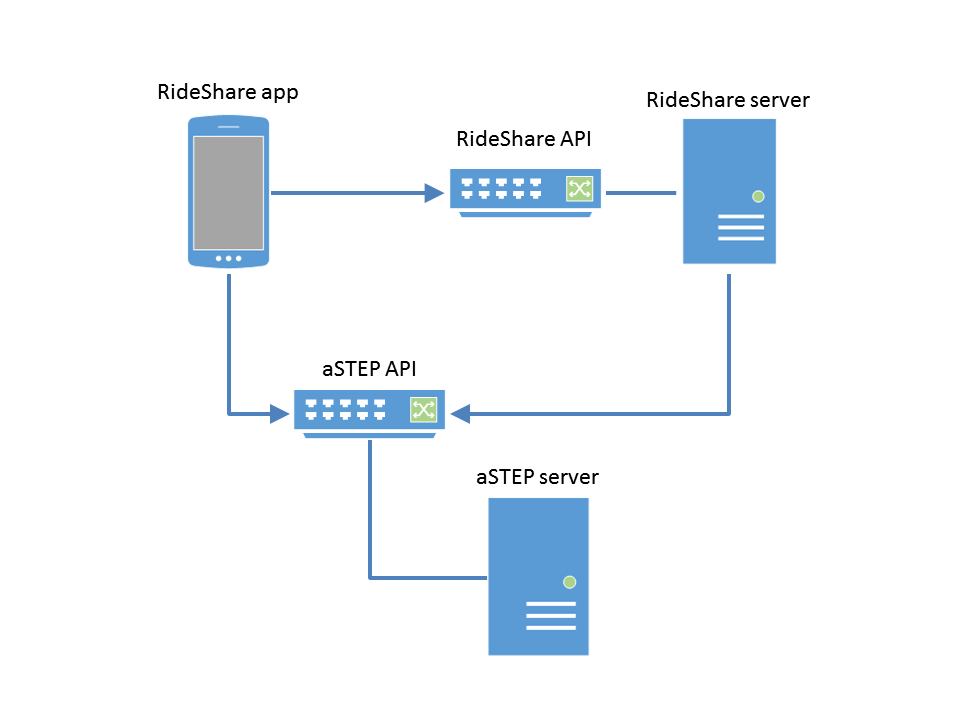
\includegraphics[width=\textwidth]{figures/SystemDesign.png}
	\caption{System design, including all major parts of the solution.}
	\label{fig:s2systemdesign}
\end{figure}


% user management responsibilities
User interface for logging in, registering a new user, edit contact information.
Through RideShare server.

% location responsibilities
Provide aSTEP system with location data directly.



% Definition of RIDESHARE(TM) server responsibilities
RideShare server..

% user management responsibilities
Relay login request from app, save and relay the token.
Because the user management system in aSTEP does only provide anything but username and password, the contact information and other data is stored on the RideShare server.


% location responsibilities
Fetch route matches for each user and store.



% Definition of aSTEP system responsibilities
aSTEP...

% user management responsibilities
Authenticate user by password.

% location responsibilities
Store locations, find stable routes, find route matches.
